%TODO cite http://blog.gdeltproject.org/gdelt-2-0-our-global-world-in-realtime/
Recent GDELT updates provide feeds with 15-minute resolution, but historical feeds offered only daily resolution. We decided for simplicity to analyze daily changes in price, taking a full day's worth of news data into account. This was most in line with testing our hypothesis, that an aggregation of topic clusters in a day's news is predictive of commodity pricing.

Our data pipeline was designed to provide day-wise parallelism over our data set in order to enable fast testing of new feature extraction methods. The raw data, as well as intermediate data, is stored in TSV ASCII format.

\subsection{Model}

%TODO cite W2V
Every news event in GDELT is stored as a row in a file for that day's report. Every set of rows may undergo a series of transformations. First, in the \textbf{preprocessing} stage, we extract relevant topic- and importance- related columns. Next, in the \textbf{expansion} stage, we project each row to a purely real space, where we use a one-hot encoding for categorical values and a Word2Vec encoding for string values, which relies on a static corpus to learn in an unsupervised manner a mapping from words to numeric vectors based on their proximity to other words every time they appear in the corpus. Finally, in the \textbf{summary} stage, this purely numeric representation of each event in a set is summarized by a static clustering classification.

The day summaries are then conglomerated in a time series $\{\textbf{d}_i\}$. For a time series of a commodity's price, $\{p_i\}$, we have the corresponding sequence of binary labels indicating whether price has increased the next day, $y_i=1_{p_{i+1}>p_i}$.

Thus, our model assumes that:
\begin{enumerate}
\item The static clustering of news topics is accurate for the future.
\item $\mathbb{P}(p_{i+1}>p_i)$ may be determined by a regression over summaries $\textbf{d}_i$. 
\end{enumerate}

Both of these are strong assumptions. The first may be weakened by adapting a dynamic clustering model, such as an infinite Gaussian Mixture Model or an HDP. The second requires $\textbf{d}_i$ to be both contain a sufficient amount of information to predict price behavior, which is a matter of appropriate feature extraction, and the assumption that we do not lose too much predictive power in summarizing a day by aggregating over the clusters to which its news events belonged to.

\subsection{Execution}

Our current implementation uses $K$-means for clustering and logistic regression for classification. We trained, validated, and sampled from the days between 2013-04-01 and 2015-07-31. Recent days were used for testing.

For our random sample, we sampled an equal number of events from each day. Even though days have variable numbers of events (and the number of reported events reduces as we go back in time), we chose this policy because the increase in news over recent years is not a property of more events occurring, but rather an increase in reporting, which should not affect the distribution of events among their hypothetical clusters of topics.

The random sample undergoes the same preprocessing and expansion pipeline as described below for the day summaries to be used in the regression, but its output is fed into a clustering model, that is then used in the main pipeline. We are forced to use a sample for tractability.

Raw data starts with 58 columns. Each day typically has 100K rows. Total size of the set is about 60GB. %TODO precise mean and stddev.

\begin{figure}[ht]
\vskip 0.2in
\begin{center}
\centerline{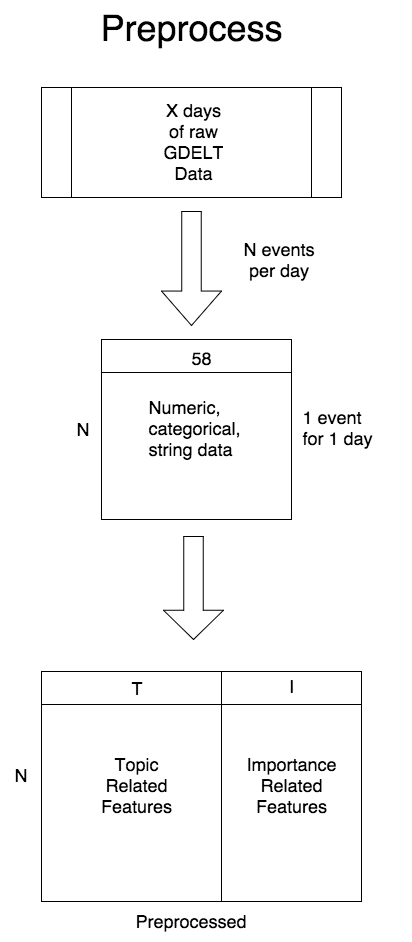
\includegraphics[scale=0.15]{images/preprocess_vertical.png}}
\caption{Preprocessing stage}
\end{center}
\vskip -0.2in
\label{fig:preprocess}
\end{figure}

After preprocessing, we are left with $T=12$ topic-related columns and $I=9$ importance columns, where the topic columns are in a compressed format, with categorical variables represented as integers and strings still as strings (though now sanitized and with stop words removed).

\begin{figure}[ht]
\vskip 0.2in
\begin{center}
\centerline{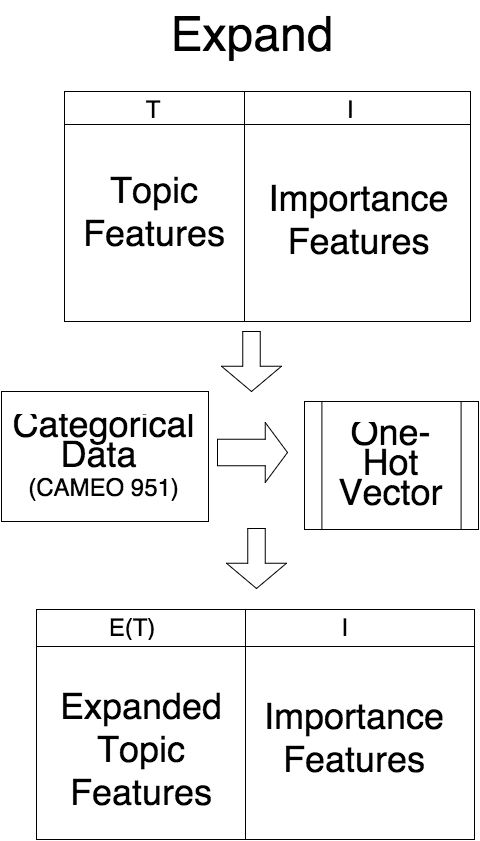
\includegraphics[scale=0.15]{images/expand_vertical.png}}
\caption{Expansion stage}
\end{center}
\vskip -0.2in
\label{fig:exapand}
\end{figure}

Expansion uses one-hot encoding on categorical features, such as the CAMEO code for the event. As mentioned before, we apply Word2Vec to expand the strings (note: not implemented yet, need larger corpus). %TODO actually do this.

%TODO mention here that we do sample-mean and sample-std-dev-based scaling, once we actually do that

\begin{figure}[ht]
\vskip 0.2in
\begin{center}
\centerline{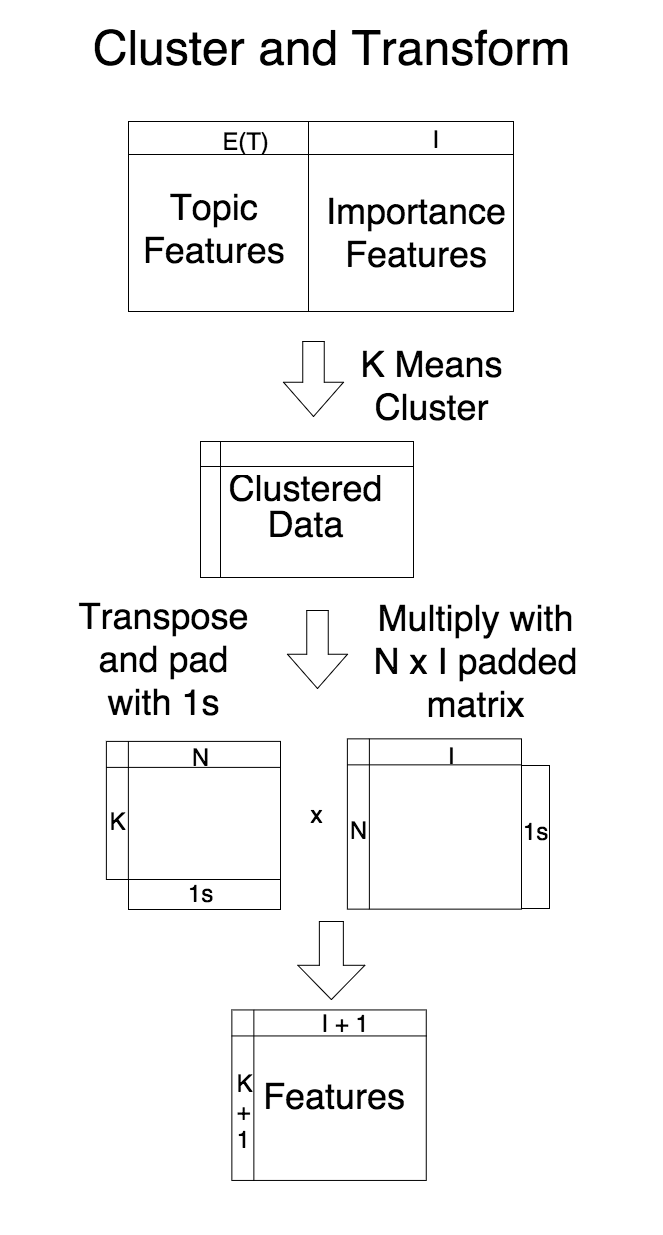
\includegraphics[scale=0.15]{images/cluster_and_transform_vertical.png}}
\caption{Summary stage}
\end{center}
\vskip -0.2in
\label{fig:summarization}
\end{figure}

The matrix multiply above conveniently extracts the sum of importance-weighted events belonging to certain topics. Note that this model is extensible to a mixture model, where each event's contribution to a topic's importance for that day is weighed by the probability of belonging to that topic's class. Furthermore, the aggregation creates a uniform description of every day, a flattened vector of dimension dependent on the cluster count.

These daily summaries were then enriched with historical pricing data before being fed into the linear model. The pricing data added was the 5, 10, and 30 day rolling average of the commodity price. %TODO hyperparam selection of rolling mean.

\subsection{Validation}

We partitioned the summarized data into training and validation sets, to train the regression's hyperparameters for regularization. This had several repercussions:
\begin{enumerate}
\item We lost a significant amount of training data. Cross-validation is not feasible because one would be attempting to guess past prices based on future data - this is incompatible with the problem of predicting tomorrow's price increase.
\item The data we lost to the validation set is more recent, so our model may be stale on current data. Is it safe to re-train a model to include the validation set's data as training data?
\end{enumerate}
